\documentclass{standalone}
\usepackage{tikz}
\usetikzlibrary{patterns, positioning}


\begin{document}
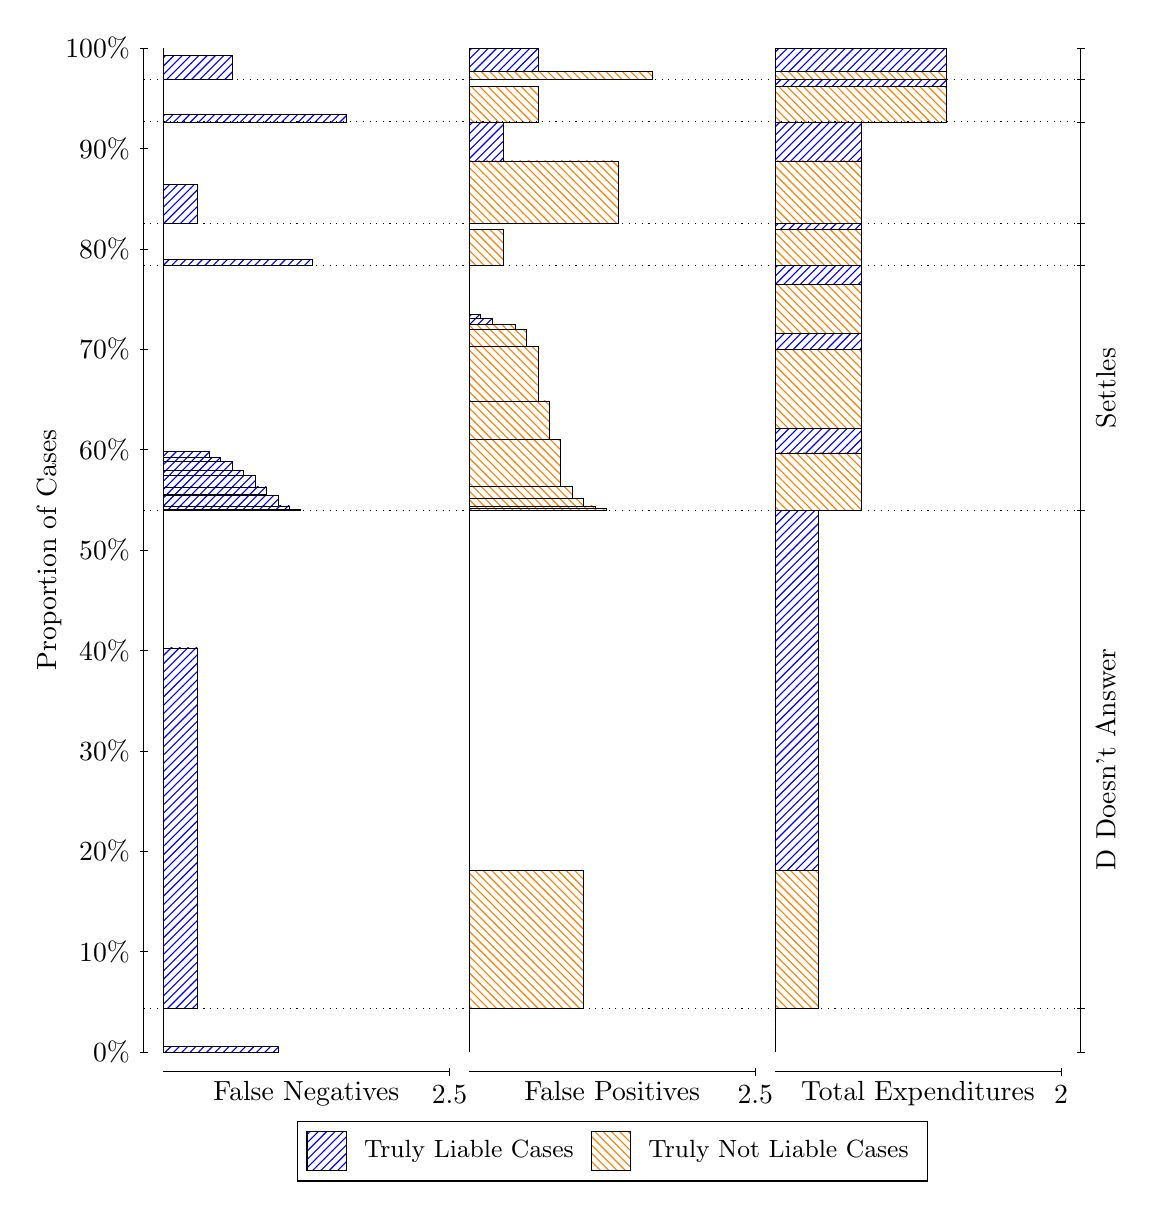
\begin{tikzpicture}
\draw[black, very thin] (1.5,1.75) -- (1.5,14.5);
\node[rotate=90, text=black, anchor=center] at (0.3, 8.125) {Proportion of Cases};
\draw[black, very thin] (1.45,1.75) -- (1.55,1.75);
\node[text=black, anchor=east] at (1.45, 1.75) {0\%};
\draw[black, very thin] (1.45,3.025) -- (1.55,3.025);
\node[text=black, anchor=east] at (1.45, 3.025) {10\%};
\draw[black, very thin] (1.45,4.3) -- (1.55,4.3);
\node[text=black, anchor=east] at (1.45, 4.3) {20\%};
\draw[black, very thin] (1.45,5.575) -- (1.55,5.575);
\node[text=black, anchor=east] at (1.45, 5.575) {30\%};
\draw[black, very thin] (1.45,6.85) -- (1.55,6.85);
\node[text=black, anchor=east] at (1.45, 6.85) {40\%};
\draw[black, very thin] (1.45,8.125) -- (1.55,8.125);
\node[text=black, anchor=east] at (1.45, 8.125) {50\%};
\draw[black, very thin] (1.45,9.4) -- (1.55,9.4);
\node[text=black, anchor=east] at (1.45, 9.4) {60\%};
\draw[black, very thin] (1.45,10.675) -- (1.55,10.675);
\node[text=black, anchor=east] at (1.45, 10.675) {70\%};
\draw[black, very thin] (1.45,11.95) -- (1.55,11.95);
\node[text=black, anchor=east] at (1.45, 11.95) {80\%};
\draw[black, very thin] (1.45,13.225) -- (1.55,13.225);
\node[text=black, anchor=east] at (1.45, 13.225) {90\%};
\draw[black, very thin] (1.45,14.5) -- (1.55,14.5);
\node[text=black, anchor=east] at (1.45, 14.5) {100\%};

\draw[black, very thin] (13.4,1.75) -- (13.4,14.5);
\draw[black, very thin] (13.35,1.75) -- (13.45,1.75);
\node[anchor=west] at (13.35, 1.75) {};
\draw[black, very thin] (13.35,2.3054) -- (13.45,2.3054);
\node[anchor=west] at (13.35, 2.3054) {};
\draw[black, very thin] (13.35,8.6289) -- (13.45,8.6289);
\node[anchor=west] at (13.35, 8.6289) {};
\draw[black, very thin] (13.35,11.738) -- (13.45,11.738);
\node[anchor=west] at (13.35, 11.738) {};
\draw[black, very thin] (13.35,12.273) -- (13.45,12.273);
\node[anchor=west] at (13.35, 12.273) {};
\draw[black, very thin] (13.35,13.562) -- (13.45,13.562);
\node[anchor=west] at (13.35, 13.562) {};
\draw[black, very thin] (13.35,14.104) -- (13.45,14.104);
\node[anchor=west] at (13.35, 14.104) {};
\draw[black, very thin] (13.35,14.5) -- (13.45,14.5);
\node[anchor=west] at (13.35, 14.5) {};

\draw[black, very thin, pattern color=blue, pattern=north east lines] (1.75,1.75) rectangle (3.2033,1.8253);
\draw[black, very thin, pattern color=orange, pattern=north west lines] (1.75,1.8253) rectangle (1.75,2.3054);
\draw[black, very thin, pattern color=blue, pattern=north east lines] (1.75,2.3054) rectangle (2.186,6.8818);
\draw[black, very thin, pattern color=orange, pattern=north west lines] (1.75,6.8818) rectangle (1.75,8.6289);
\draw[black, very thin, pattern color=blue, pattern=north east lines] (1.75,8.6289) rectangle (3.494,8.6435);
\draw[black, very thin, pattern color=blue, pattern=north east lines] (1.75,8.6435) rectangle (3.3487,8.6847);
\draw[black, very thin, pattern color=blue, pattern=north east lines] (1.75,8.6847) rectangle (3.2033,8.8199);
\draw[black, very thin, pattern color=blue, pattern=north east lines] (1.75,8.8199) rectangle (3.058,8.8361);
\draw[black, very thin, pattern color=blue, pattern=north east lines] (1.75,8.8361) rectangle (3.058,8.9262);
\draw[black, very thin, pattern color=blue, pattern=north east lines] (1.75,8.9262) rectangle (2.9127,9.074);
\draw[black, very thin, pattern color=blue, pattern=north east lines] (1.75,9.074) rectangle (2.7673,9.1396);
\draw[black, very thin, pattern color=blue, pattern=north east lines] (1.75,9.1396) rectangle (2.622,9.2475);
\draw[black, very thin, pattern color=blue, pattern=north east lines] (1.75,9.2475) rectangle (2.4767,9.2986);
\draw[black, very thin, pattern color=blue, pattern=north east lines] (1.75,9.2986) rectangle (2.3313,9.3799);
\draw[black, very thin, pattern color=orange, pattern=north west lines] (1.75,9.3799) rectangle (1.75,11.738);
\draw[black, very thin, pattern color=blue, pattern=north east lines] (1.75,11.738) rectangle (3.6393,11.819);
\draw[black, very thin, pattern color=orange, pattern=north west lines] (1.75,11.819) rectangle (1.75,12.273);
\draw[black, very thin, pattern color=blue, pattern=north east lines] (1.75,12.273) rectangle (2.186,12.767);
\draw[black, very thin, pattern color=orange, pattern=north west lines] (1.75,12.767) rectangle (1.75,13.562);
\draw[black, very thin, pattern color=blue, pattern=north east lines] (1.75,13.562) rectangle (4.0753,13.658);
\draw[black, very thin, pattern color=orange, pattern=north west lines] (1.75,13.658) rectangle (1.75,14.104);
\draw[black, very thin, pattern color=blue, pattern=north east lines] (1.75,14.104) rectangle (2.622,14.405);
\draw[black, very thin, pattern color=orange, pattern=north west lines] (1.75,14.405) rectangle (1.75,14.5);
\draw[black, very thin, pattern color=orange, pattern=north west lines] (5.6333,1.75) rectangle (5.6333,2.2302);
\draw[black, very thin, pattern color=blue, pattern=north east lines] (5.6333,2.2302) rectangle (5.6333,2.3054);
\draw[black, very thin, pattern color=orange, pattern=north west lines] (5.6333,2.3054) rectangle (7.0867,4.0526);
\draw[black, very thin, pattern color=blue, pattern=north east lines] (5.6333,4.0526) rectangle (5.6333,8.6289);
\draw[black, very thin, pattern color=orange, pattern=north west lines] (5.6333,8.6289) rectangle (7.3773,8.6577);
\draw[black, very thin, pattern color=orange, pattern=north west lines] (5.6333,8.6577) rectangle (7.232,8.6844);
\draw[black, very thin, pattern color=orange, pattern=north west lines] (5.6333,8.6844) rectangle (7.0867,8.7847);
\draw[black, very thin, pattern color=orange, pattern=north west lines] (5.6333,8.7847) rectangle (6.9413,8.9284);
\draw[black, very thin, pattern color=orange, pattern=north west lines] (5.6333,8.9284) rectangle (6.796,9.5307);
\draw[black, very thin, pattern color=orange, pattern=north west lines] (5.6333,9.5307) rectangle (6.6507,10.019);
\draw[black, very thin, pattern color=orange, pattern=north west lines] (5.6333,10.019) rectangle (6.5053,10.707);
\draw[black, very thin, pattern color=orange, pattern=north west lines] (5.6333,10.707) rectangle (6.36,10.925);
\draw[black, very thin, pattern color=orange, pattern=north west lines] (5.6333,10.925) rectangle (6.2147,10.987);
\draw[black, very thin, pattern color=blue, pattern=north east lines] (5.6333,10.987) rectangle (5.924,11.068);
\draw[black, very thin, pattern color=blue, pattern=north east lines] (5.6333,11.068) rectangle (5.7787,11.119);
\draw[black, very thin, pattern color=blue, pattern=north east lines] (5.6333,11.119) rectangle (5.6333,11.738);
\draw[black, very thin, pattern color=orange, pattern=north west lines] (5.6333,11.738) rectangle (6.0693,12.192);
\draw[black, very thin, pattern color=blue, pattern=north east lines] (5.6333,12.192) rectangle (5.6333,12.273);
\draw[black, very thin, pattern color=orange, pattern=north west lines] (5.6333,12.273) rectangle (7.5227,13.068);
\draw[black, very thin, pattern color=blue, pattern=north east lines] (5.6333,13.068) rectangle (6.0693,13.562);
\draw[black, very thin, pattern color=orange, pattern=north west lines] (5.6333,13.562) rectangle (6.5053,14.008);
\draw[black, very thin, pattern color=blue, pattern=north east lines] (5.6333,14.008) rectangle (5.6333,14.104);
\draw[black, very thin, pattern color=orange, pattern=north west lines] (5.6333,14.104) rectangle (7.9587,14.199);
\draw[black, very thin, pattern color=blue, pattern=north east lines] (5.6333,14.199) rectangle (6.5053,14.5);
\draw[black, very thin, pattern color=orange, pattern=north west lines] (9.5167,1.75) rectangle (9.5167,2.2302);
\draw[black, very thin, pattern color=blue, pattern=north east lines] (9.5167,2.2302) rectangle (9.5167,2.3054);
\draw[black, very thin, pattern color=orange, pattern=north west lines] (9.5167,2.3054) rectangle (10.062,4.0526);
\draw[black, very thin, pattern color=blue, pattern=north east lines] (9.5167,4.0526) rectangle (10.062,8.6289);
\draw[black, very thin, pattern color=orange, pattern=north west lines] (9.5167,8.6289) rectangle (10.607,9.3583);
\draw[black, very thin, pattern color=blue, pattern=north east lines] (9.5167,9.3583) rectangle (10.607,9.6651);
\draw[black, very thin, pattern color=orange, pattern=north west lines] (9.5167,9.6651) rectangle (10.607,10.671);
\draw[black, very thin, pattern color=blue, pattern=north east lines] (9.5167,10.671) rectangle (10.607,10.878);
\draw[black, very thin, pattern color=orange, pattern=north west lines] (9.5167,10.878) rectangle (10.607,11.501);
\draw[black, very thin, pattern color=blue, pattern=north east lines] (9.5167,11.501) rectangle (10.607,11.738);
\draw[black, very thin, pattern color=orange, pattern=north west lines] (9.5167,11.738) rectangle (10.607,12.192);
\draw[black, very thin, pattern color=blue, pattern=north east lines] (9.5167,12.192) rectangle (10.607,12.273);
\draw[black, very thin, pattern color=orange, pattern=north west lines] (9.5167,12.273) rectangle (10.607,13.068);
\draw[black, very thin, pattern color=blue, pattern=north east lines] (9.5167,13.068) rectangle (10.607,13.562);
\draw[black, very thin, pattern color=orange, pattern=north west lines] (9.5167,13.562) rectangle (11.697,14.008);
\draw[black, very thin, pattern color=blue, pattern=north east lines] (9.5167,14.008) rectangle (11.697,14.104);
\draw[black, very thin, pattern color=orange, pattern=north west lines] (9.5167,14.104) rectangle (11.697,14.199);
\draw[black, very thin, pattern color=blue, pattern=north east lines] (9.5167,14.199) rectangle (11.697,14.5);
\draw[black, dotted] (1.5,2.3054) -- (13.4,2.3054);
\draw[black, dotted] (1.5,8.6289) -- (13.4,8.6289);
\draw[black, dotted] (1.5,11.738) -- (13.4,11.738);
\draw[black, dotted] (1.5,12.273) -- (13.4,12.273);
\draw[black, dotted] (1.5,13.562) -- (13.4,13.562);
\draw[black, dotted] (1.5,14.104) -- (13.4,14.104);
\draw[black, very thin] (1.75,1.5) -- (5.3833,1.5);
\node[text=black, anchor=north] at (3.5667, 1.5) {False Negatives};
\draw[black, very thin] (5.3833,1.45) -- (5.3833,1.55);
\node[text=black, anchor=north] at (5.3833, 1.45) {2.5};

\draw[black, very thin] (5.6333,1.5) -- (9.2667,1.5);
\node[text=black, anchor=north] at (7.45, 1.5) {False Positives};
\draw[black, very thin] (9.2667,1.45) -- (9.2667,1.55);
\node[text=black, anchor=north] at (9.2667, 1.45) {2.5};

\draw[black, very thin] (9.5167,1.5) -- (13.15,1.5);
\node[text=black, anchor=north] at (11.333, 1.5) {Total Expenditures};
\draw[black, very thin] (13.15,1.45) -- (13.15,1.55);
\node[text=black, anchor=north] at (13.15, 1.45) {2};


\node[text=black, centered, rotate=90] at (13.72, 5.4672) {D Doesn't Answer};
\node[text=black, centered, rotate=90] at (13.72, 10.183) {Settles};





\draw (7.449999999999999,1.5) node[draw=none] (baseCoordinate) {};
\begin{scope}[align=center]
        \matrix[scale=0.5, draw=black, below=0.5cm of baseCoordinate, nodes={draw}, column sep=0.1cm]{
            \node[rectangle, draw, minimum width=0.5cm, minimum height=0.5cm, pattern color=blue, pattern=north east lines] {}; &
            \node[draw=none, font=\small, text=black] (B) {Truly Liable Cases}; &
            \node[rectangle, draw, minimum width=0.5cm, minimum height=0.5cm, pattern color=orange, pattern=north west lines] {}; &
            \node[draw=none, font=\small, text=black] (B) {Truly Not Liable Cases}; \\
            };
\end{scope}

\end{tikzpicture}
\end{document}